\documentclass{article}
\usepackage{tikz}
\usetikzlibrary{calc}

\begin{document}

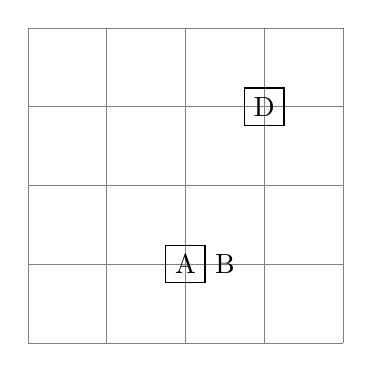
\begin{tikzpicture}
    \draw [help lines] (0,0) grid (4,4);
    \node[draw] (A) at (2,1) {A};
    \node[draw] (D) at (3,3) {D};
    \path let \p1 = (A),
    \p2=(D),\n3={(\x2+\x1)/2} in node at (\n3,\y1) {B};
\end{tikzpicture}

\end{document}